\documentclass{article}
\usepackage{iclr2027_conference}
\usepackage{times}
\usepackage{amsmath,amssymb,amsthm,mathtools}
\usepackage{booktabs,multirow,array}
\usepackage{graphicx}
\usepackage[table]{xcolor}
\usepackage{microtype}
\usepackage{xspace}
\usepackage{hyperref}
\usepackage{url}

\newcommand{\method}{\textsc{EESD}\xspace}
\newcommand{\eed}{\textsc{EED}\xspace}
\newcommand{\fix}{\textsc{Fix}\xspace}
\newcommand{\regress}{\textsc{Regress}\xspace}
\newcommand{\preserve}{\textsc{Preserve}\xspace}
\newcommand{\unresolved}{\textsc{Unresolved}\xspace}
\newcommand{\R}{\mathbb{R}}
\newcommand{\E}{\mathbb{E}}
\newcommand{\KL}{\mathrm{KL}}
\newcommand{\ind}{\mathbb{I}}
\newtheorem{proposition}{Proposition}
\newtheorem{corollary}{Corollary}

\definecolor{cardblue}{RGB}{235,244,252}
\definecolor{cardgreen}{RGB}{237,248,241}
\definecolor{cardpurple}{RGB}{245,240,250}
\definecolor{cardorange}{RGB}{252,245,235}
\definecolor{posgreen}{RGB}{226,242,231}
\definecolor{negred}{RGB}{249,231,231}
\definecolor{neutralgray}{RGB}{243,244,246}

\hypersetup{colorlinks=true,linkcolor=blue,citecolor=blue,urlcolor=blue,
  pdftitle={How Much Evidence Should a Self-Correction Carry? Adaptive Dirichlet Evidence for Self-Distillation},
  pdfauthor={Anonymous authors},pdfsubject={ICLR 2027 submission}}
\title{\raggedright How Much Evidence Should a Self-Correction Carry? Adaptive Dirichlet Evidence for Self-Distillation}
\author{Anonymous authors}
\date{}
% \iclrfinalcopy

\begin{document}
\maketitle
% Keep the review header when using newer installed fancyhdr versions.
\lhead{Under review as a conference paper at ICLR 2027}



\begin{abstract}
Language-model agents can generate, execute, and revise their own solutions, creating supervision for self-improvement. A correction's apparent quality, however, need not reveal how concentrated its external support is. We introduce \emph{Effective-Evidence Self-Distillation} (\method), which separates relative transition support from an effective pseudo-count mass derived from normalized execution relevance. A Dirichlet posterior converts these quantities into an uncertainty-penalized correction weight for KL-anchored self-distillation. Under a symmetric prior, changing mass preserves category ordering, while effective mass cannot increase the supervised coefficient relative to matched fixed-mass weighting. Across four model--domain history sweeps, increasing visible observations from one to eight reduces EED future-outcome NLL by $55.0$--$59.3\%$. At eight observations, EED also achieves lower NLL than fixed mass in all four comparisons. In a matched DeepSeek/RunBugRun study, the predictors agree in argmax on all 3,000 examples, with the largest NLL gain in the most concentrated relevance bin. The complete learning update achieves its largest observed downstream gain on DeepSeek/CodeARC, raising all-tests Pass@1 from $15.0\%$ to $20.4\%$. These results connect an explicit evidence decomposition to probability estimation and correction learning.
\end{abstract}





\section{Introduction}

Language-model agents increasingly operate in environments that return objective feedback: compilers, unit tests, simulators, APIs, and interactive tools. This has made self-correction practical. Self-Refine and Reflexion reuse model-generated feedback or reflection at inference time \citep{madaan2023selfrefine,shinn2023reflexion}; Self-Debugging revises programs after observing execution behavior \citep{chen2024selfdebug}; and execution-guided repair, search, and verification systems use tests to select or refine candidate programs \citep{ni2023lever,tang2024rex,li2025codeprm,li2025sstar,tao2026execcritic}. These methods answer an increasingly well-studied question: \emph{can the model produce a better next answer after feedback?}

A second line of work asks which self-generated trajectories are safe or useful to learn from. Correctness filtering retains successful trajectories, reward-based methods favor higher-reward behavior, and confidence-aware self-training distinguishes trajectories that share an observed outcome \citep{jiang2025importance,jang2025corepo,yang2025dnpo}. These signals assess trajectory quality, but need not separately represent two properties of the execution record: \emph{which before/after transitions the observations support} and \emph{how much total evidence supports that direction}. The question is how the weight is constructed, not whether its final representation is scalar.

\begin{figure*}[t]
\centering
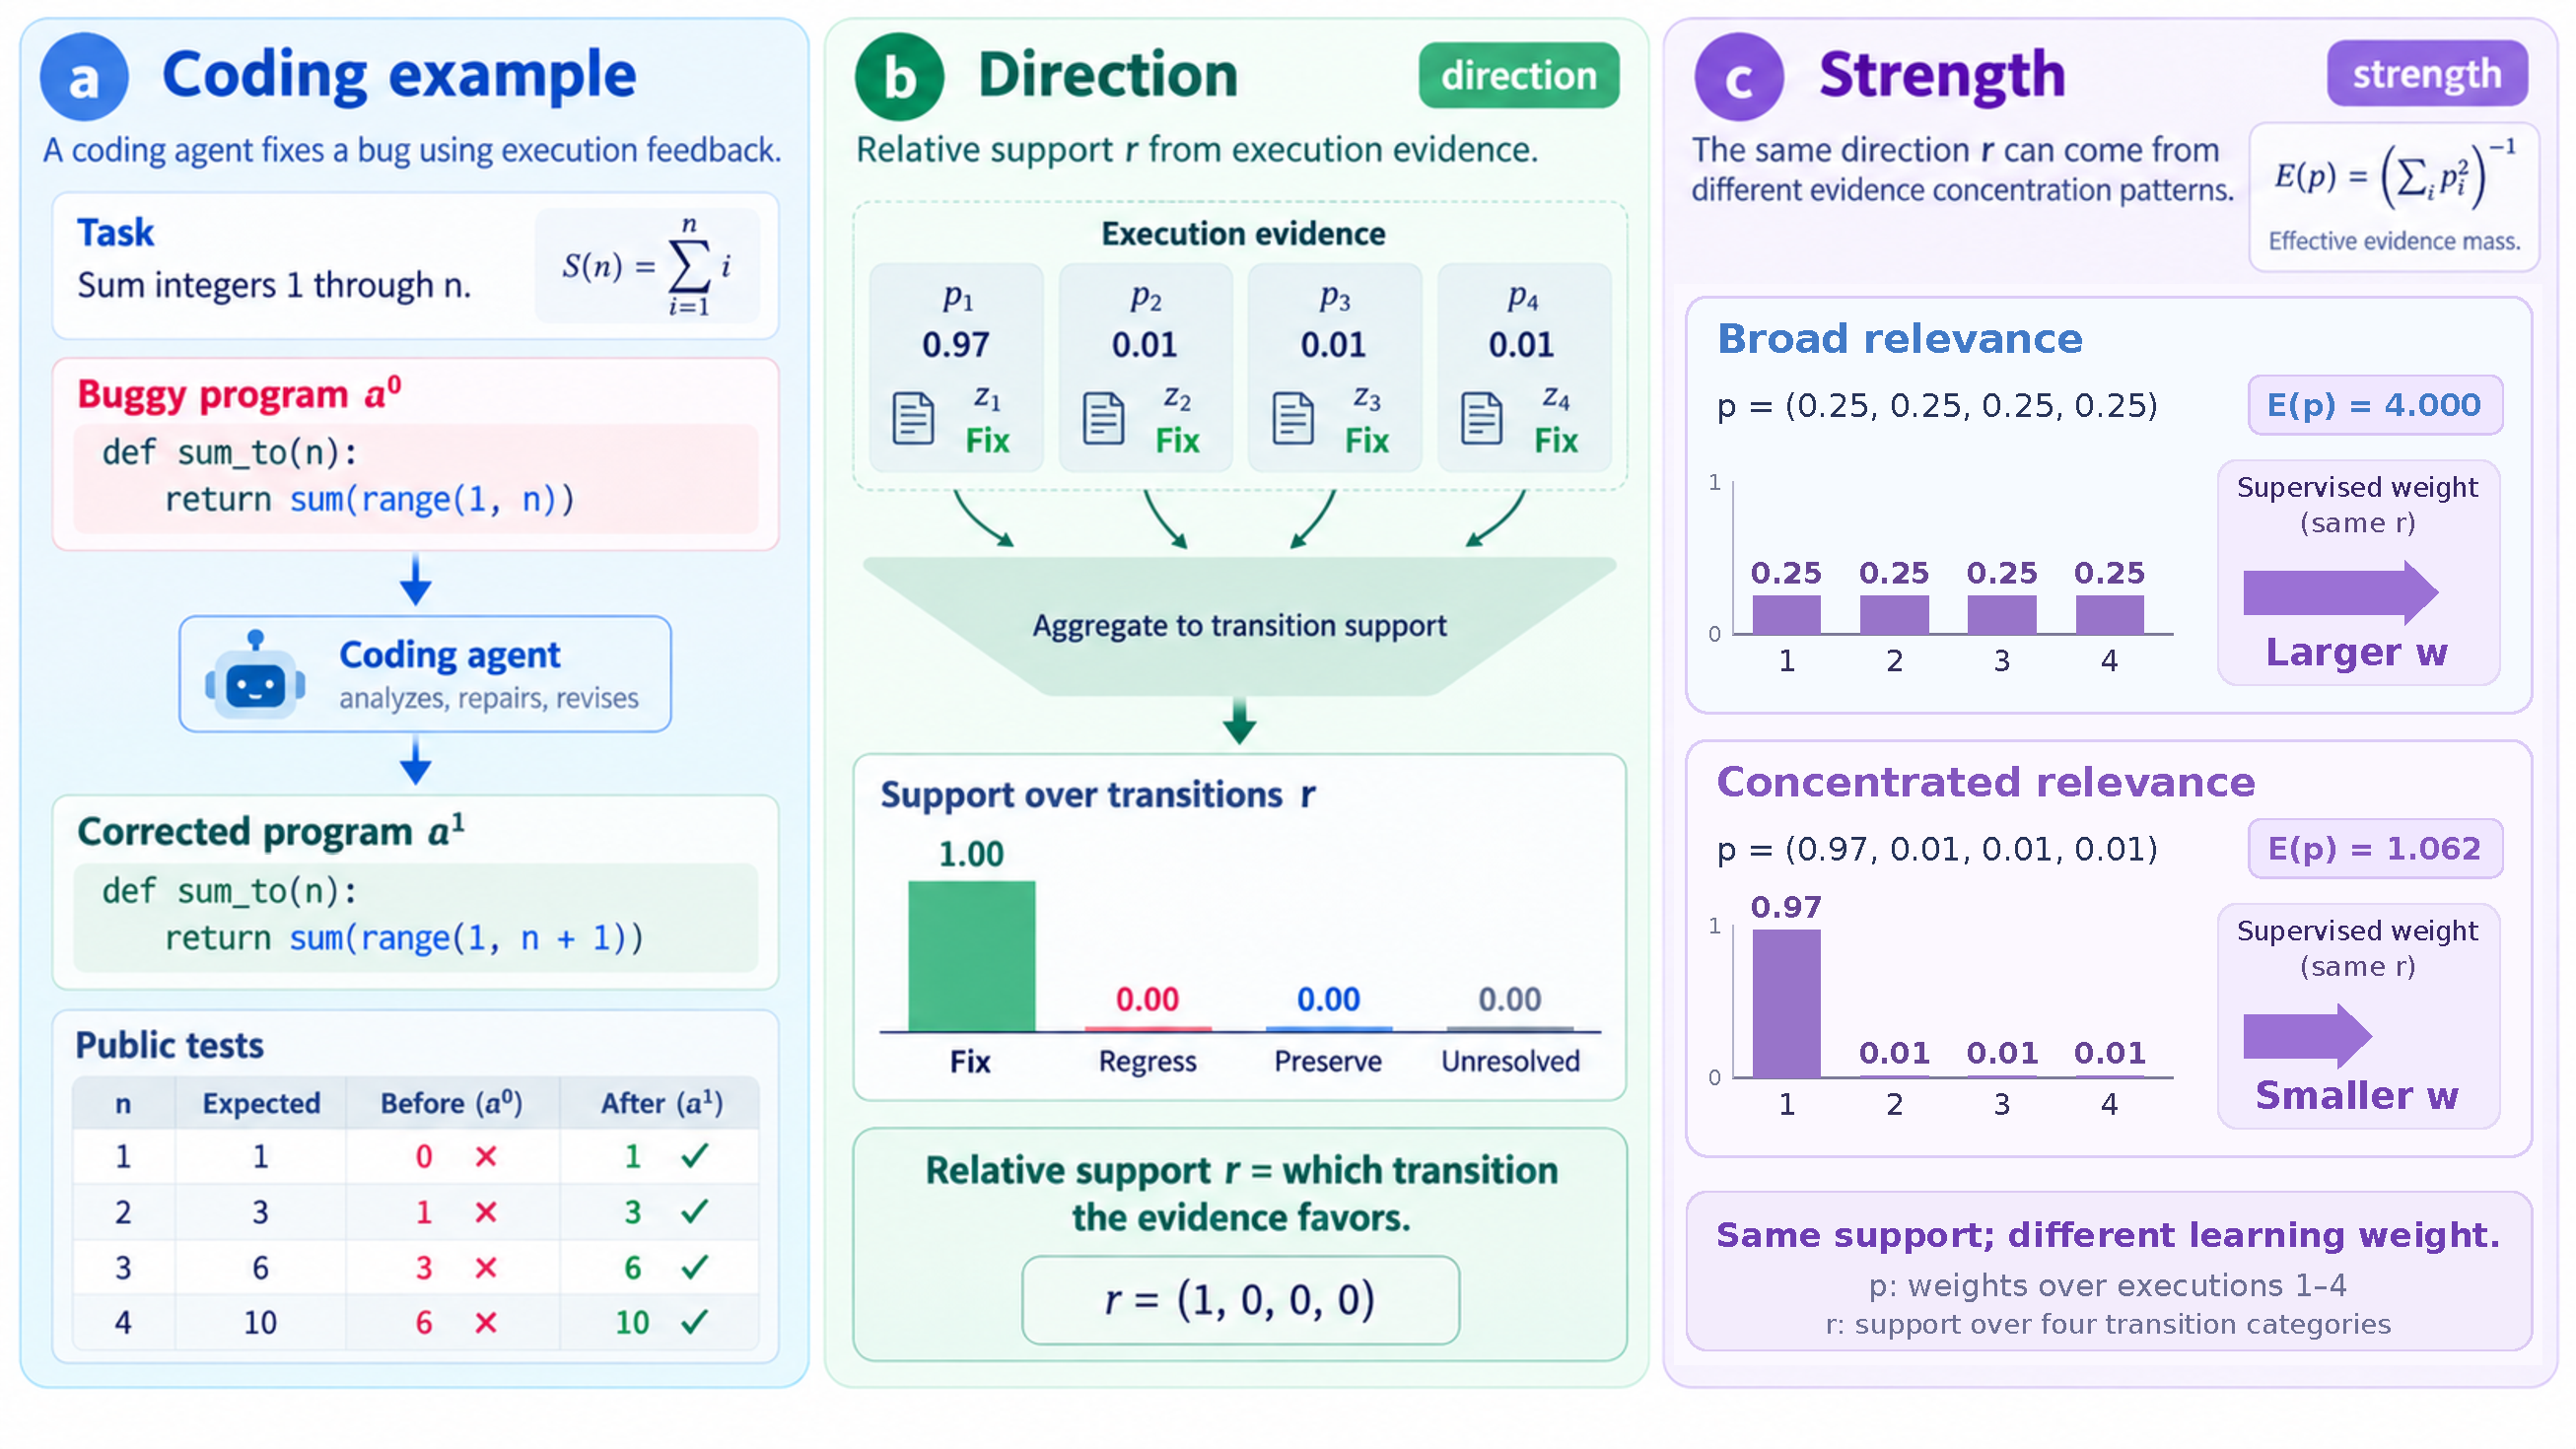
\includegraphics[width=\linewidth]{figures/intro.pdf}
\caption{\textbf{Direction and strength in a coding correction.}
(a) Fixing an off-by-one range error changes four public executions from fail to pass.
(b) Aggregating execution relevance by transition gives $r=(1,0,0,0)$: all support favors \fix.
(c) The same transitions under uniform and concentrated relevance give $E(p)=4.000$ and $1.062$; at fixed prior and utility settings, they yield different supervised weights.
The $p$ bars index executions, whereas the $r$ bars index transition categories. Relevance weights are stipulated for this analytical illustration, not measured on a benchmark.}
\label{fig:problem}
\end{figure*}

Figure~\ref{fig:problem} illustrates the distinction through an off-by-one repair. Extending a Python range endpoint makes all four public executions pass, so relative support is $r=(1,0,0,0)$ under either relevance pattern. Uniform relevance assigns comparable weight to every execution and gives $E(p)=4$; concentrated relevance $p=(0.97,0.01,0.01,0.01)$ gives $E(p)\approx1.062$. A fixed-mass control restores total mass to four in both cases. \method instead lets relevance concentration change the supervised weight while retaining the same correction target. The relevance vectors are stipulated to isolate this distinction; the code and before/after outputs make its meaning concrete.

The problem becomes more consequential when corrections are written back into model parameters. A mistaken inference-time correction affects one answer; an over-weighted training correction changes the policy that will generate future answers and future training data. We therefore ask: \emph{given a self-generated correction, how much should the next policy learn from the execution evidence supporting it?}

We introduce \emph{Effective-Evidence Self-Distillation} (\method), a probabilistic trust layer between correction and learning. Given nonnegative relevance scores $s_i$, \method normalizes them into $p$. Relative support $r$ describes \emph{what} transition categories the observations favor, while
$E(p)=(\sum_i p_i^2)^{-1}$ describes \emph{how much} pseudo-count mass that support contributes. A Dirichlet posterior produces an uncertainty-penalized correction utility; its positive part scales correction cross-entropy while a KL term anchors the student to the entering policy. The upstream correction generator and relevance estimator remain modular: the contribution is how their execution record is converted into a learning coefficient.

Our contributions are:
\begin{enumerate}
\item We formulate correction-level \emph{direction--strength separation}: distinguishing relative execution support from the total evidence mass assigned to that support.
\item We introduce \eed, which converts relevance concentration into adaptive Dirichlet pseudo-count mass, and connect its posterior utility to KL-anchored LoRA self-distillation. We characterize count recovery, ordering invariance, and the resulting control of the supervised coefficient.
\item We evaluate the construction through visible-history scaling, a matched-mass mechanism study with fixed argmax, and one-round fresh program generation across multiple models and domains.
\end{enumerate}

\begin{table*}[t]
\centering
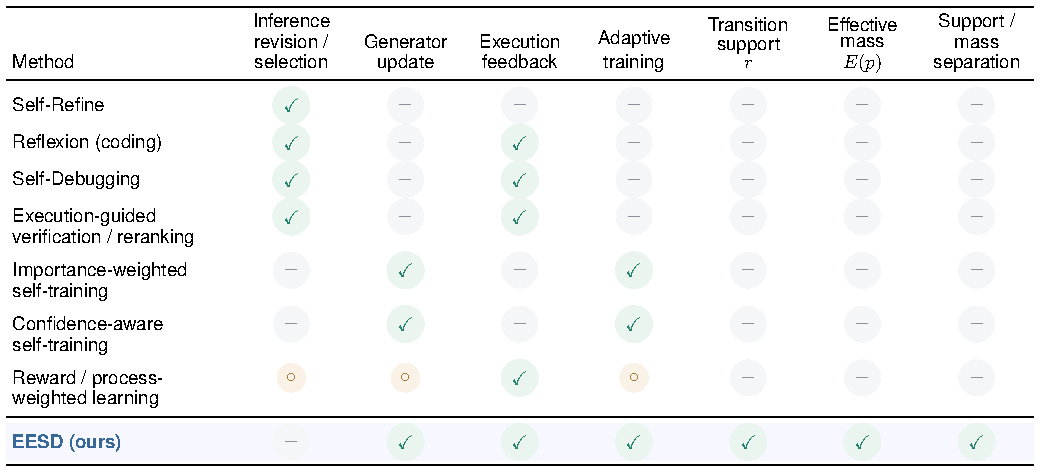
\includegraphics[width=\linewidth]{figures/liter.pdf}
\caption{\textbf{Positioning by the role of feedback.} $\checkmark$: explicit use; --: absent in the cited formulation; $\circ$: varies within a grouped family. Generator updates exclude auxiliary-verifier training. Adaptive training includes filtering, preferences, and reward weighting. The last three columns concern our correction-level support--mass construction, not uncertainty modeling in general. This is a conceptual comparison, not a benchmark result; representative methods are discussed in Section~\ref{sec:related}.}
\label{tab:positioning}
\end{table*}

\section{Related Work}
\label{sec:related}

Table~\ref{tab:positioning} positions \method relative to representative
self-correction and self-training approaches. The central distinction
is between improving an answer, assessing its suitability for learning,
and determining how much execution evidence supports the resulting
update.

\paragraph{Self-correction and execution-guided repair.}
A broad line of work studies how language models can improve an answer
after observing feedback. Self-Refine iteratively revises outputs using
model-generated critiques, while Reflexion stores verbal feedback from
previous attempts to guide subsequent decisions
\citep{madaan2023selfrefine,shinn2023reflexion}. Reflexion can use external execution feedback in its coding setting; Self-Debugging likewise uses execution behavior to revise programs
\citep{chen2024selfdebug}. Execution-guided verification and reranking
use execution results to assess and select candidate programs
\citep{ni2023lever,li2025sstar}; related repair-search and critic-based
systems use feedback to guide further revisions
\citep{tang2024rex,tao2026execcritic}. LEVER trains an auxiliary verifier rather than the code-generating policy. REx already uses Bayesian beliefs, but to allocate repair-search effort rather than correction-level training weights. These approaches illustrate how
external execution evidence can support inference-time correction
and candidate selection. Our question begins after a correction has
been obtained: rather than introducing another repair or reranking
procedure, \method determines how strongly that correction should
contribute to a parameter update.

\paragraph{Learning from self-generated corrections.}
Self-training turns generated trajectories into parameter updates,
making the reliability of each trajectory consequential beyond a
single inference episode. Correctness filtering retains successful
samples, while importance-weighted self-training adjusts the selection
or contribution of generated examples under distributional mismatch
\citep{jiang2025importance}. Confidence-aware self-training uses model
or reasoning confidence to distinguish trajectories that may share
the same observed outcome \citep{jang2025corepo}. Reward / process-weighted
learning uses outcome rewards or intermediate-step assessments: CodePRM learns a process evaluator, whereas ExecCritic also trains repair agents \citep{li2025codeprm,tao2026execcritic}. Iterative
preference-learning methods study how to sustain improvement across
updates \citep{yang2025dnpo}. These families, grouped in
Table~\ref{tab:positioning}, refine which trajectories are selected
or how they influence learning. \method focuses on a different
quantity within each correction record: the amount of execution
evidence supporting its relative transition preferences. Its final
training weight is also scalar, but is derived from separately
represented evidence direction and evidence amount, rather than
identified with correctness, reward, or model confidence alone.

\paragraph{Evidential uncertainty and effective sample size.}
Our probabilistic construction connects to two established statistical
ideas. Dirichlet models distinguish categorical probabilities from
distributional concentration and have been used to represent evidential
uncertainty \citep{sensoy2018evidential}. The inverse squared
concentration of normalized weights is also a standard
effective-sample-size functional \citep{martino2017ess}. We introduce
neither component. Instead, \method uses relative transition support
$r$ to represent evidence direction and effective mass $E(p)$ to
represent the amount of relevance-weighted support. Their
direction--strength separation determines the Dirichlet pseudo-count
update and its uncertainty-penalized correction utility. This utility
sets the supervised coefficient in KL-anchored self-distillation:
for \method, adaptive training in Table~\ref{tab:positioning} refers
to this correction-specific coefficient, not the norm of an optimizer step. The distinction is therefore the explicit
execution-to-learning decomposition, rather than the use of
uncertainty modeling or adaptive weighting in general.




\section{Effective-Evidence Self-Distillation}
\label{sec:method}

\method converts execution feedback into a correction-specific training weight. The key is to separate \emph{relative transition support} from \emph{total evidence mass}, then use both to determine how strongly to learn from a correction.

\begin{figure*}[t]
\centering
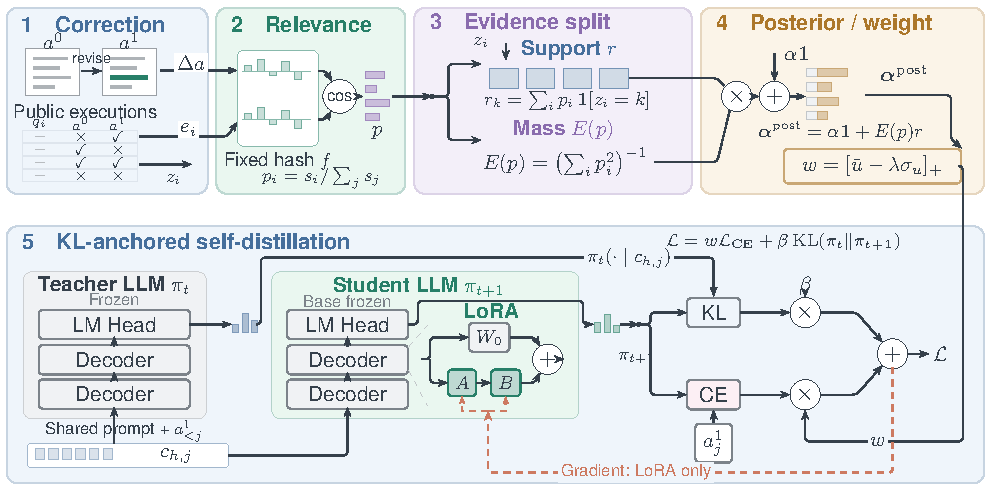
\includegraphics[width=1\linewidth]{figures/flow.pdf}
\caption{\textbf{Effective-Evidence Self-Distillation.} The public correction record yields $p$ and transition labels $z_i$. Parallel support and mass summaries form a pseudo-count posterior and weight $w$. Teacher and student consume the same prompt and past correction tokens; the current target $a^1_j$ enters CE only. Teacher probabilities enter KL, not the student input. Only CE is weighted by $w$, and only LoRA receives gradients. Decoder stacks and the low-rank inset are schematic, not a target-layer specification.}
\label{fig:method}
\end{figure*}

\subsection{Correction evidence}
\label{sec:problem}

For a programming task $x$, policy $\pi_t$ produces an initial program $a^0$, and an upstream repair procedure returns a correction $a^1$. Both programs are evaluated on the same $n\ge1$ public executions $\{q_i\}_{i=1}^{n}$, yielding before/after outcomes $(o_i^0,o_i^1)$. Let $h$ denote this correction record. Each outcome pair defines a transition
\begin{equation}
z_i\in\{\fix,\regress,\preserve,\unresolved\},
\end{equation}
corresponding to fail$\rightarrow$pass, pass$\rightarrow$fail, pass$\rightarrow$pass, and fail$\rightarrow$fail, respectively.

Each execution receives a relevance score $s_i\ge0$, with $\sum_i s_i>0$. Define
\begin{align}
p_i &= \frac{s_i}{\sum_j s_j},
\label{eq:normalized-relevance}\\
r_k &= \sum_i p_i\ind[z_i=k].
\label{eq:relative-support}
\end{align}
The four-vector $r$ describes which transitions the observations support. Here direction denotes category ordering, not a parameter-space gradient. Our implementation obtains $s_i$ from a frozen lexical kernel comparing the code change with public execution descriptors; Appendix~\ref{app:architecture} gives the details.

\subsection{From effective evidence to correction utility}

Our fixed-mass control uses $c_k^{\mathrm{fixed}}=nr_k$, preserving relative support while assigning every record of length $n$ the same total mass. \eed replaces this nominal mass with
\begin{align}
E(p) &= \left(\sum_i p_i^2\right)^{-1},
\label{eq:effective-evidence}\\
\alpha_k^{\mathrm{post}} &= \alpha+E(p)r_k,
\qquad \alpha>0,
\label{eq:posterior}
\end{align}
and defines $\theta\mid h\sim\mathrm{Dir}(\boldsymbol\alpha^{\mathrm{post}})$. Thus $r$ allocates pseudo-counts across transitions, while $E(p)$ sets their total mass. We have $1\le E(p)\le n$; uniform relevance gives $E(p)p_i=1$ and recovers ordinary counts. The Dirichlet is a working uncertainty model conditional on relevance: its pseudo-count mass measures concentration, not the number of statistically independent tests.

To reward fixes and penalize regressions, set $v=(1,-1,0,0)$. Writing $\alpha_0=\sum_k\alpha_k^{\mathrm{post}}$ and $\mu_k=\alpha_k^{\mathrm{post}}/\alpha_0$, the posterior utility moments are
\begin{align}
\bar u &= \E[v^\top\theta]
=\mu_{\fix}-\mu_{\regress},
\label{eq:utility-mean}\\
\sigma_u^2 &=
\frac{\mu_{\fix}+\mu_{\regress}-\bar u^2}{\alpha_0+1}.
\label{eq:utility-variance}
\end{align}
The correction weight is
\begin{equation}
w(h)=\left[\bar u-\lambda\sigma_u\right]_+,
\qquad \lambda\ge0,
\label{eq:utility}
\end{equation}
where $[a]_+=\max(a,0)$. The uncertainty penalty reduces the supervised contribution of corrections with less decisive posterior utility; nonpositive utility yields zero supervised weight. It is not a calibrated confidence bound.

For the all-\fix example in Figure~\ref{fig:problem}, $\alpha=0.1$ and $\lambda=0.5$ give weights $0.832$ and $0.542$ for uniform and concentrated relevance. The matched fixed-mass control assigns $0.832$ to both. Appendix~\ref{app:coding-illustration} gives the calculation. These are supervised coefficients, not measured performance or optimizer-step norms.

\subsection{KL-anchored self-distillation}

The student learns from $a^1$ while a frozen copy of $\pi_t$ supplies a forward-KL anchor:
\begin{equation}
\mathcal L_{\method}(h)
=
w(h)\mathcal L_{\mathrm{CE}}(h)
+\beta D_{\mathrm{KL}}^{(h)}(\pi_t\Vert\pi_{t+1}).
\label{eq:eesd-loss}
\end{equation}
Here $\mathcal L_{\mathrm{CE}}$ is correction cross-entropy, and $D_{\mathrm{KL}}^{(h)}$ is forward KL averaged over the same response-token prefixes. Only the supervised term is weighted by $w(h)$. We train LoRA parameters with the quantized base frozen; token-level definitions and fixed hyperparameters are in Appendix~\ref{app:architecture}.

\label{sec:theory}
\begin{proposition}[Outcome ordering and correction weight]
\label{prop:direction-strength}
Fix $r$, a symmetric prior $\alpha>0$, $\lambda\ge0$, and $v=(1,-1,0,0)$. Replace $E(p)$ by any mass $\tau>0$ in Equations~\ref{eq:posterior}--\ref{eq:utility}. The posterior mean satisfies
\begin{equation}
\mu_k(\tau)
=\gamma(\tau)r_k+\frac{1-\gamma(\tau)}{4},
\qquad
\gamma(\tau)=\frac{\tau}{4\alpha+\tau}.
\label{eq:shrinkage}
\end{equation}
Consequently, category ordering and the argmax set are invariant to $\tau$. Moreover, the correction weight $w_\tau$ is nondecreasing in $\tau$, so
\begin{equation}
w_{E(p)}\le w_n.
\label{eq:weight-attenuation}
\end{equation}
\end{proposition}
Thus effective evidence cannot increase the supervised coefficient relative to matched fixed-mass weighting. Probability estimates can nevertheless change without changing categorical predictions; whether this improves NLL depends on the observed outcome. Appendix~\ref{app:proofs} gives the proofs and the log-loss characterization.




\section{Experiments}
\label{sec:experiments}

We evaluate three questions. \textbf{RQ1} examines whether additional visible executions improve outcome prediction. \textbf{RQ2} isolates how effective mass changes predictive probabilities at fixed relative support. \textbf{RQ3} tests the complete correction-learning update through fresh program generation. Figures~\ref{fig:history-scaling} and~\ref{fig:performance-summary} organize these measurements, with full numerical reports in the appendix.

\subsection{Experimental setup}

\paragraph{Tasks and models.}
We use RunBugRun and CodeARC, together with APPS Replay and CodeContests Replay \citep{runbugrun,codearc}. RunBugRun contains executable buggy programs; CodeARC tests program synthesis from behavioral observations. All results use the recorded source populations and execution budgets below; the replay domains use controlled synthesis extensions rather than official leaderboard settings. The CodeARC evaluation also differs from its original interactive differential-testing protocol \citep{codearc}. The downstream matrix covers Qwen2.5-Coder-7B-Instruct, DeepSeek-Coder-6.7B-Instruct, and Gemma-3-4B-it, with 500 primary sources per model--domain cell.

\paragraph{Measurements and comparisons.}
The prediction studies measure future-outcome negative log-likelihood (NLL) and categorical accuracy. The history sweep compares fixed mass $n$ with effective mass $E(p)$ as visible history grows. A separate matched comparison holds relative support and predictor parameters fixed, changing only the pseudo-count mass. Downstream evaluation generates one fresh candidate per source after one update; all-tests Pass@1 requires passing all ten evaluator tests. It compares full \method (\texttt{eesd\_full}) with the unchanged entering policy (\texttt{no\_update}). The paired effect, in percentage points, is
\begin{equation}
\Delta_{\mathrm{pp}}=100\bigl[S(\texttt{eesd\_full})-S(\texttt{no\_update})\bigr],
\label{eq:downstream-delta}
\end{equation}
where $S$ is the fraction of solved sources. We retain the reported paired 95\% intervals from 10,000 whole-source bootstrap draws. These quantify source-level uncertainty for the evaluated policies. Hidden outcomes are evaluation signals, not inputs to the evidence scorer. Fresh generation means a new completion on the recorded source population; protocol and replication details are in Appendix~\ref{app:protocol}.

\paragraph{Training and hardware.}
We adapt LoRA parameters on a frozen 4-bit NF4 base with bfloat16 computation. The correction scorer uses $\alpha=0.1$ and $\lambda=0.5$; the forward-KL coefficient is $\beta=0.03$. Experiments use NVIDIA RTX A6000 hardware with 48\,GB nominal memory per GPU. Evidence weights are computed from public records before student fitting, and the frozen entering policy supplies the KL reference. Appendix~\ref{app:architecture} specifies the relevance kernel, response-token objective, and optimization settings.

\subsection{RQ1: Does additional visible evidence improve prediction?}
\label{sec:rq1}
\label{sec:history-scaling}

We first ask whether the available executions carry useful predictive information. Figure~\ref{fig:history-scaling} varies visible history size over $n\in\{1,2,4,8\}$ for DeepSeek and Qwen on RunBugRun and CodeARC. Here $n$ counts observations, not training rounds. This study establishes the value of accumulating execution history before examining how its mass should be assigned.

\paragraph{Prediction improves with longer histories.}
EED NLL decreases at every measured step in all four model--domain cells. On RunBugRun, the endpoint changes are $0.4696\rightarrow0.2114$ for DeepSeek and $0.4737\rightarrow0.2113$ for Qwen. On CodeARC, they are $0.7103\rightarrow0.2892$ and $0.7785\rightarrow0.3415$. Table~\ref{tab:history-summary} expresses these changes as relative NLL reductions of $55.0$--$59.3\%$. Categorical accuracy improves as well: by $2.5$ and $1.9$ percentage points on RunBugRun, and by $5.5$ and $6.1$ points on CodeARC, respectively. Additional history therefore benefits both the probability assigned to the observed outcome and the categorical prediction. These measurements concern the outcome estimator; the learned policy is evaluated separately in RQ3.

\paragraph{Effective mass adds a distinct comparison.}
Fixed-mass prediction also benefits from additional observations. At $n=8$, EED further reduces NLL relative to Fixed in all four cells, as summarized in Figure~\ref{fig:performance-summary}(a): $0.0046$ and $0.0075$ on RunBugRun, and $0.0113$ and $0.0024$ on CodeARC, for DeepSeek and Qwen respectively. These are absolute NLL differences, not accuracy percentage points. At $n=1$, the two constructions coincide because $p_1=1$ and $E(p)=n=1$; differences at shorter histories are generally small. Figure~\ref{fig:history-scaling} and Appendix~\ref{app:history-size} retain the complete trajectories. Increasing $n$ can change both relative support and effective mass, so this sweep should be distinguished from the fixed-support comparison that follows.

\begin{figure*}[t]
\centering
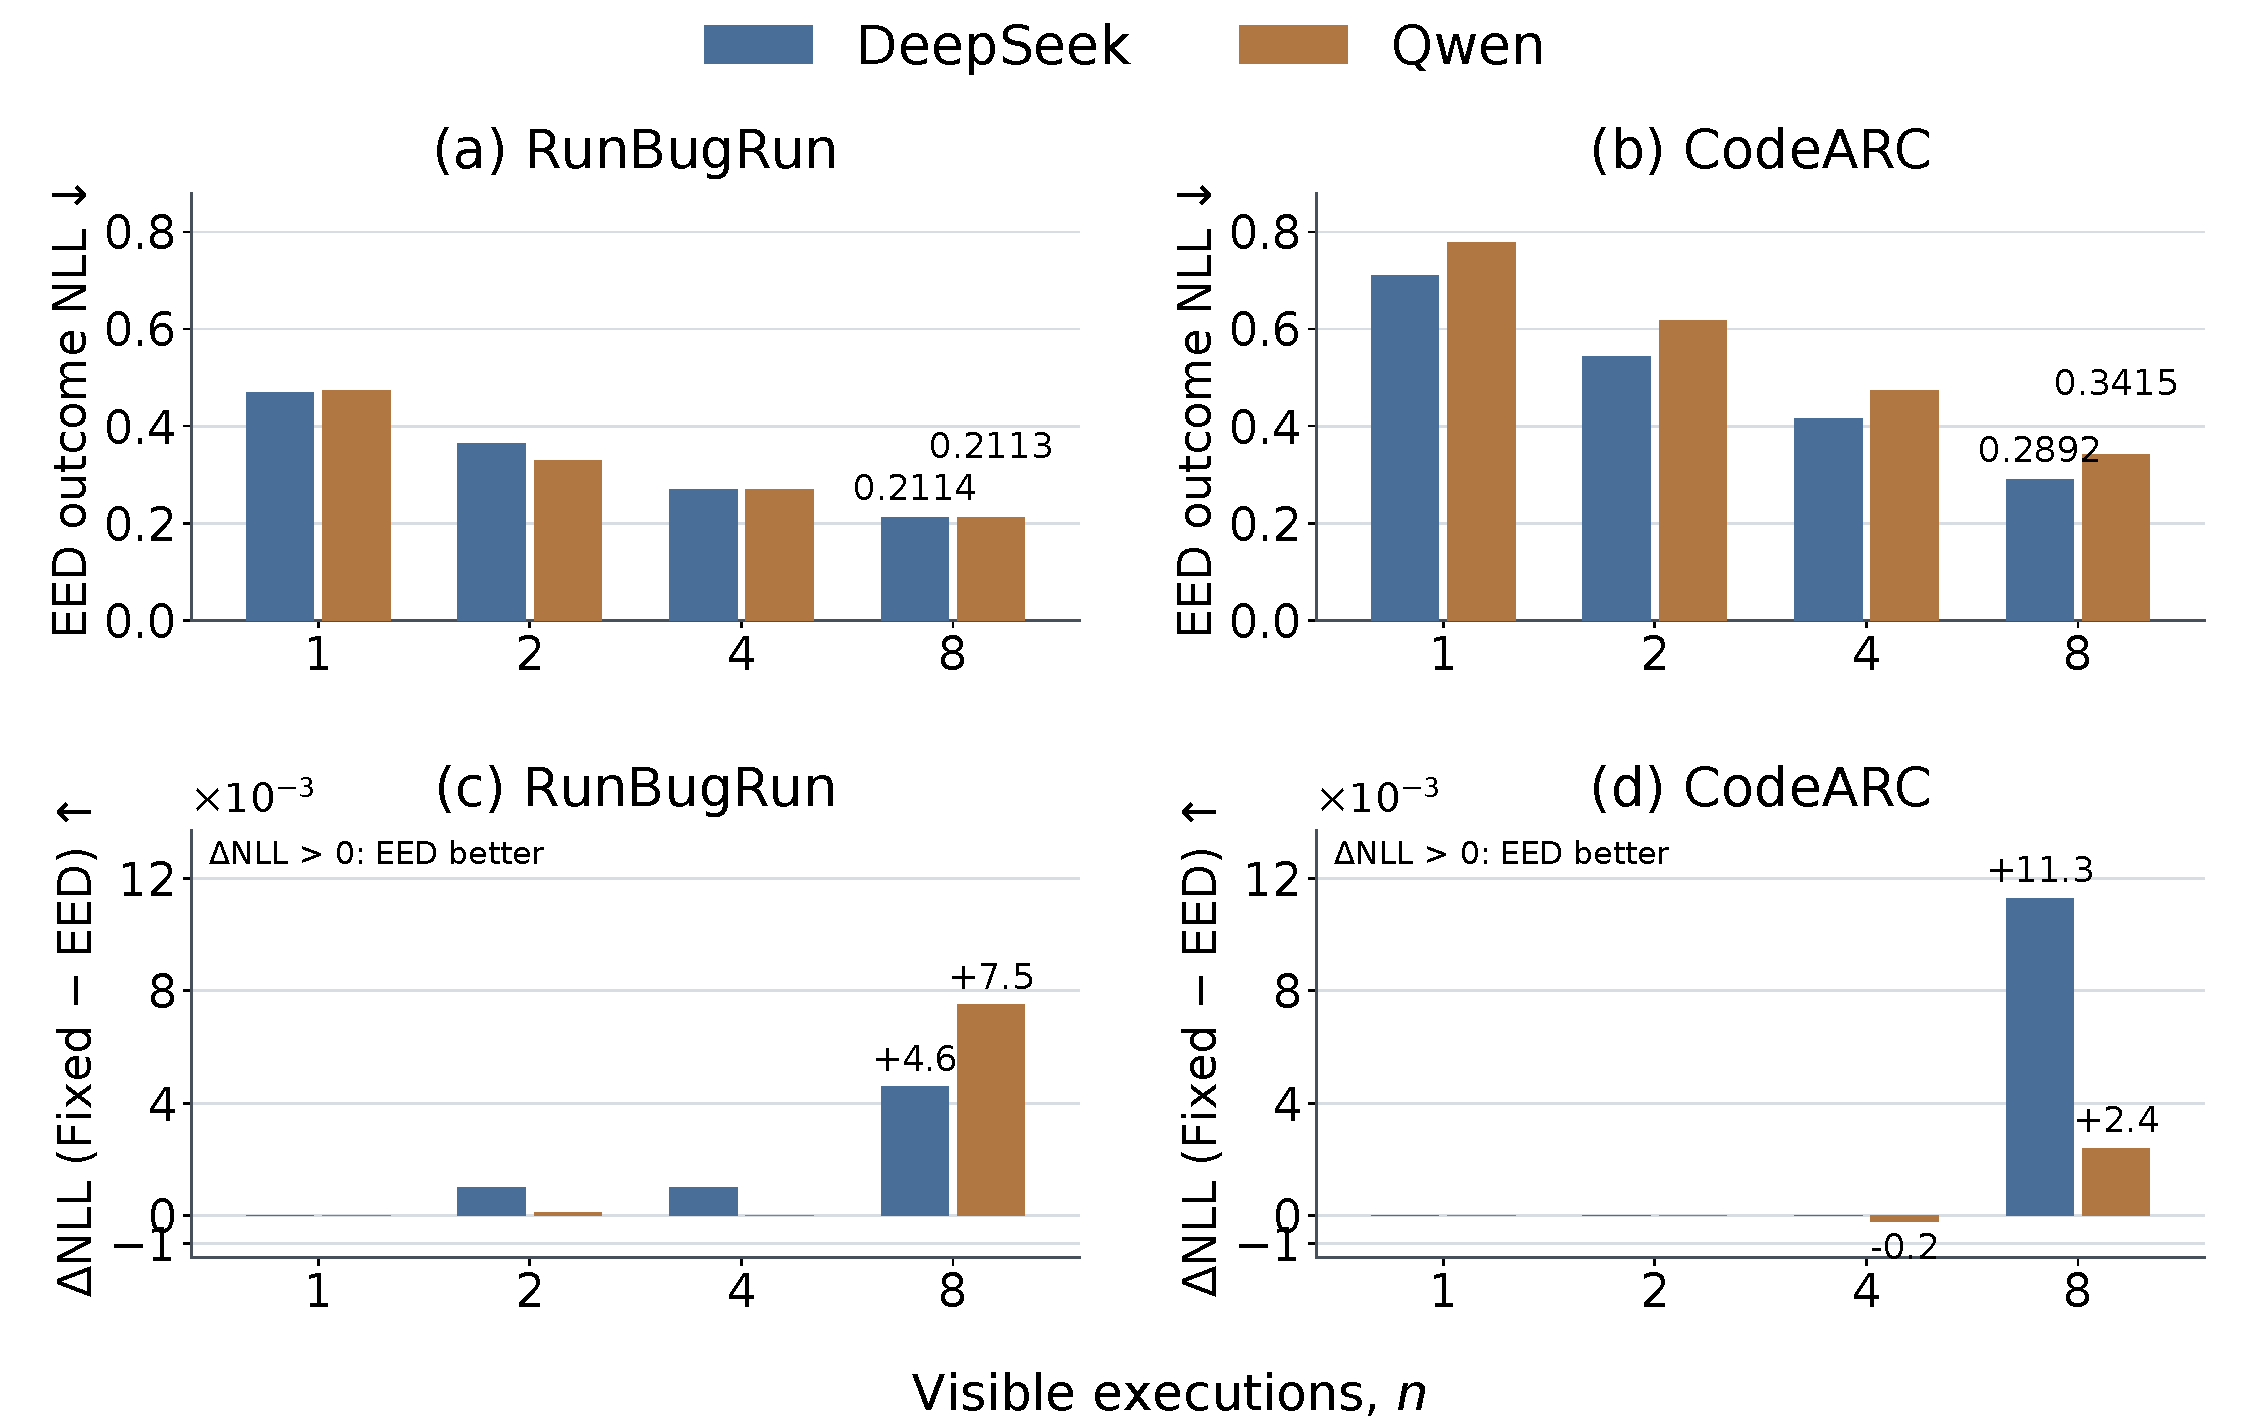
\includegraphics[width=1\linewidth]{figures/exp1.pdf}
\caption{\textbf{History size and effective evidence answer different questions.} (a,b) EED future-outcome NLL: lower is better. (c,d) $\Delta\mathrm{NLL}=\mathrm{NLL}_{\mathrm{Fixed}}-\mathrm{NLL}_{\mathrm{EED}}$: higher is better, in units of $10^{-3}$. All panels use $n=1,2,4,8$ visible observations, not training rounds. Differences are calculated from the four-decimal measurements in Table~\ref{tab:history-full}. The matched-parameter comparison is reported separately in Section~\ref{sec:rq2}.}
\label{fig:history-scaling}
\end{figure*}

\begin{table*}[t]
\centering
\small
\caption{\textbf{Endpoint summary of the EED history sweep.} NLL reduction and accuracy change compare $n=1$ with $n=8$; $\Delta\mathrm{NLL}_{8}=\mathrm{NLL}_{\mathrm{Fixed}}-\mathrm{NLL}_{\mathrm{EED}}$ at $n=8$. The reductions are calculated from the reported rounded measurements.}
\setlength{\tabcolsep}{6pt}
\begin{tabular}{llcccc}
\toprule
Benchmark & Backbone & EED NLL $1\!\rightarrow\!8$ & Reduction (\%) & Acc. change (pp) & $\Delta\mathrm{NLL}_{8}$ $\uparrow$ \\
\midrule
RunBugRun & DeepSeek 6.7B & $0.4696\!\rightarrow\!0.2114$ & 55.0 & +2.5 & +0.0046 \\
RunBugRun & Qwen2.5 7B & $0.4737\!\rightarrow\!0.2113$ & 55.4 & +1.9 & +0.0075 \\
CodeARC & DeepSeek 6.7B & $0.7103\!\rightarrow\!0.2892$ & 59.3 & +5.5 & +0.0113 \\
CodeARC & Qwen2.5 7B & $0.7785\!\rightarrow\!0.3415$ & 56.1 & +6.1 & +0.0024 \\
\bottomrule
\end{tabular}
\label{tab:history-summary}
\end{table*}

\subsection{RQ2: Does effective evidence change strength without changing direction?}
\label{sec:rq2}

The primary matched comparison uses DeepSeek/RunBugRun with the same relative support and effective-arm hyperparameters for both predictors. Only total pseudo-count mass changes. Their categorical argmax predictions agree on all 3,000 future-outcome examples, while effective mass reduces aggregate NLL by $0.00609$ with a 95\% source-bootstrap interval of $[0.00211,0.01075]$. Thus better probability estimates do not require changing the selected category. The ordering argument in Proposition~\ref{prop:direction-strength} applies to any categorical predictor with a symmetric prior, as detailed in Appendix~\ref{app:logloss}; the four-transition utility is the separate training construction.

\paragraph{The largest gain occurs under concentrated relevance.}
Table~\ref{tab:concentration} and Figure~\ref{fig:performance-summary}(b) divide the matched comparison into three effective-mass bins. The NLL reduction is $0.0159$ for $1\le E(p)<2$, $0.0077$ for $2\le E(p)<3$, and $0.0018$ for $3\le E(p)\le4$. The corresponding mean masses retain $37.8\%$, $63.0\%$, and $92.0\%$ of the nominal count of four (Appendix~\ref{app:derived-summaries}). In this comparison, the largest predictive benefit is associated with the largest reduction in pseudo-count mass. When support is already broadly distributed, effective and nominal mass are closer and the observed difference is smaller.

The intervention neither finds another candidate nor supplies additional executions. It changes shrinkage toward the symmetric prior while retaining the relative support and its category ordering. This is the probability-level signature targeted by the method: the favored outcome can remain fixed while the confidence assigned to it changes. The mass fractions describe pseudo-counts, not measured optimizer-step sizes.

\begin{table}[t]
\centering
\small
\caption{\textbf{Concentration-stratified matched-mass comparison.} Primary DeepSeek/RunBugRun comparison. Gain is fixed-mass NLL minus EED NLL. Both predictors agree in argmax on all 3,000 examples.}
\setlength{\tabcolsep}{7pt}
\begin{tabular}{lccc}
\toprule
Effective-mass bin & Examples & Mean $E(p)$ & NLL gain $\uparrow$ \\
\midrule
$[1,2)$ & 568 & 1.511 & \textbf{+0.0159} \\
$[2,3)$ & 815 & 2.521 & +0.0077 \\
$[3,4]$ & 1617 & 3.681 & +0.0018 \\
\bottomrule
\end{tabular}
\label{tab:concentration}
\end{table}

\paragraph{From probability estimates to learning.}
The matched study tests the evidence estimator rather than policy adaptation. For training, the posterior is further mapped to a correction-specific utility and supervised coefficient. Proposition~\ref{prop:direction-strength} characterizes this mapping; RQ3 examines the complete resulting update. The other recorded mechanism repetitions and their intervals are provided in Appendix~\ref{app:mechanism-full}, separately from the history sweep. The log-loss analysis in Appendix~\ref{app:logloss} explains why a change in mass need not have the same benefit for every outcome.

\subsection{RQ3: Does correction learning improve fresh generation?}
\label{sec:rq3}

We now move from outcome prediction to the code-generating policy. Each evaluated program is freshly sampled after learning, rather than chosen by reranking an existing candidate bank. Figure~\ref{fig:performance-summary}(c) presents four selected model--domain contrasts against the unchanged policy; Appendix~\ref{app:full-matrix} reports the complete twelve-cell evaluation. The displayed contrasts are the cells with positive point estimates, not an aggregate over the matrix.

\paragraph{The clearest gain is on DeepSeek/CodeARC.}
All-tests Pass@1 rises from $75/500$ ($15.0\%$) to $102/500$ ($20.4\%$), a net increase of 27 solved sources. The paired improvement is $+5.4$ percentage points, with a 95\% source-bootstrap interval of $[+2.8,+8.0]$. This result concerns complete programs passing all ten evaluator tests, not individual test outcomes or the accuracy of an auxiliary predictor. It demonstrates a benefit of the complete correction-learning update in this model--domain setting.

\paragraph{Further gains appear on RunBugRun and CodeContests Replay.}
DeepSeek increases from $184/500$ to $198/500$ on RunBugRun ($+2.8$ points), and Qwen increases from $228/500$ to $240/500$ ($+2.4$ points). DeepSeek also increases from $18/500$ to $24/500$ on CodeContests Replay ($+1.2$ points). These correspond to 14, 12, and 6 additional solved sources in the respective aggregate counts. Their paired intervals include zero, so they provide positive point estimates rather than independent claims of statistically resolved improvement. The full matrix shows that the effect remains model--domain dependent.

\begin{figure*}[t]
\centering
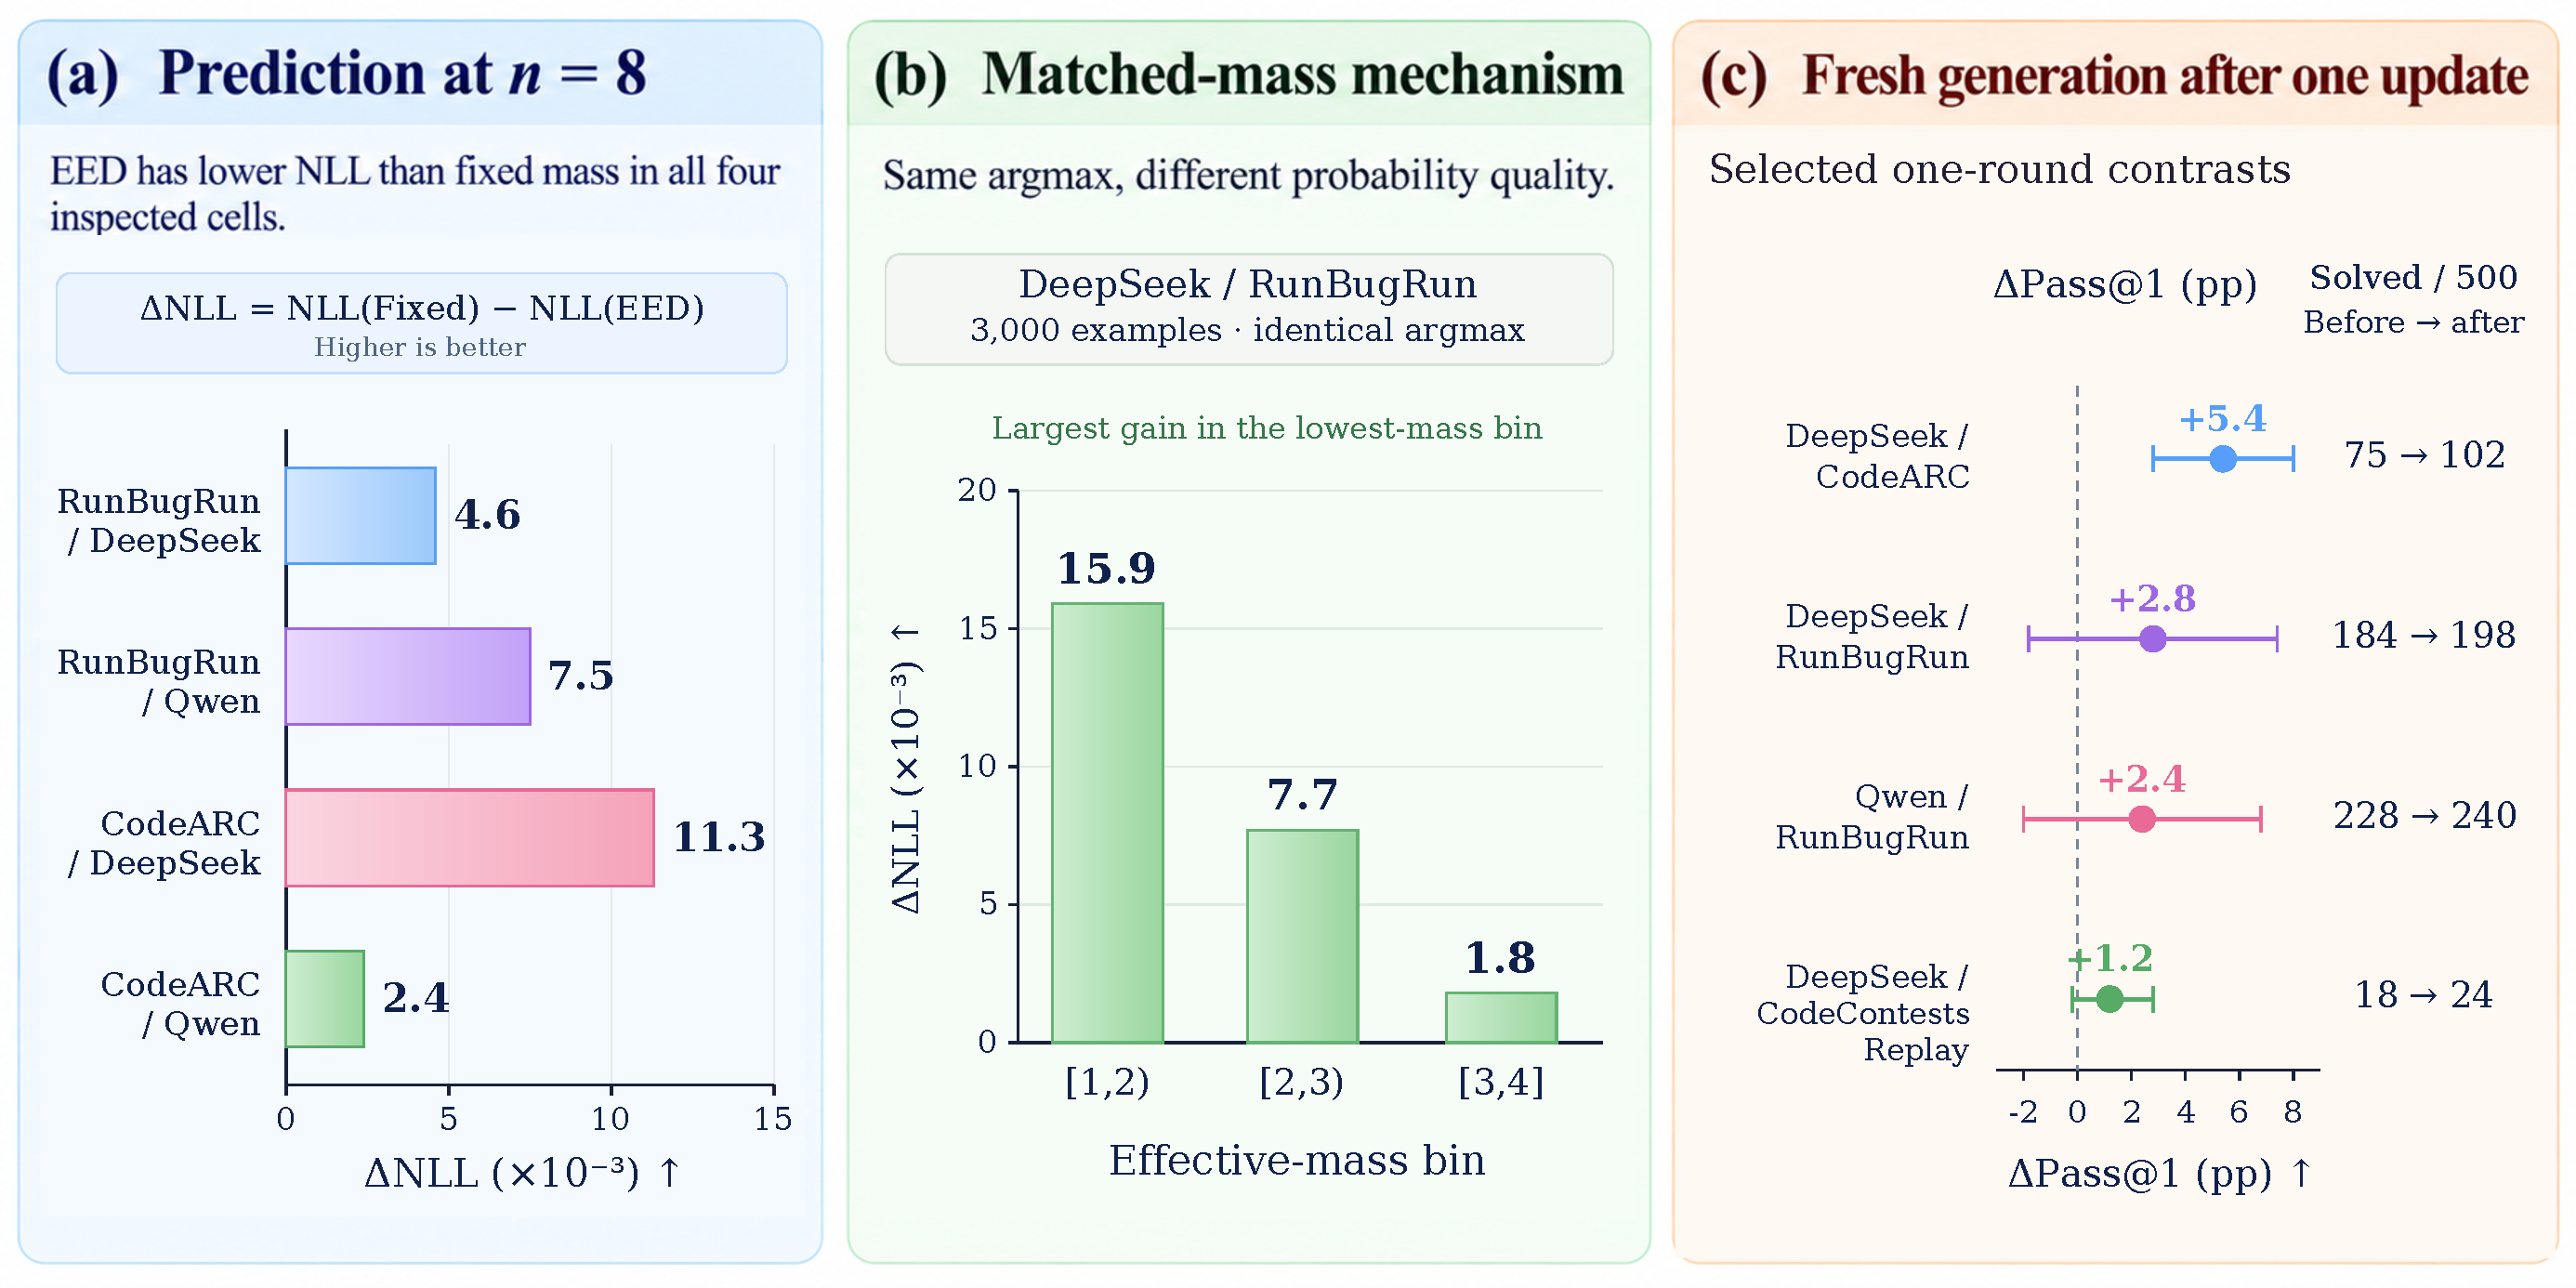
\includegraphics[width=\linewidth]{figures/performance_summary.pdf}
\caption{\textbf{Prediction and fresh-generation performance.}
(a) Fixed-minus-EED NLL at $n=8$ in the four history-sweep cells.
(b) The matched DeepSeek/RunBugRun comparison by effective-mass bin; argmax agrees on all 3,000 examples. Both NLL panels use units of $10^{-3}$ and positive values favor EED.
(c) Four selected one-round contrasts against \texttt{no\_update}, with paired 95\% source-bootstrap intervals and solved counts out of 500. The complete model--domain evaluation is in Table~\ref{tab:full-downstream}.}
\label{fig:performance-summary}
\end{figure*}

Together, the studies examine successive parts of the evidence-to-learning path: additional observations improve prediction, matched mass changes probability estimates without changing category ordering, and the complete weighted update improves fresh generation in several model--domain settings. The downstream comparison assesses \method as a whole; the controlled probability-level result is not a component-level training ablation. Appendix~\ref{app:future} specifies the comparisons represented in the current result matrix.

\section{Limitations}

The evaluation focuses on executable coding tasks and one-round adaptation. More expressive relevance estimators can replace the frozen lexical kernel without changing the construction, but effective mass measures concentration rather than test independence. The reported downstream comparison evaluates the complete update; component attribution and source-disjoint transfer require separate evidence. Broader tasks and repeated adaptation remain natural extensions. Full results and replication details are provided in the appendix.

\section{Conclusion}
\label{sec:conclusion}

\method separates what execution evidence supports from how much pseudo-count mass it contributes, then uses posterior utility to weight KL-anchored self-distillation. The analysis connects this decomposition to category-order invariance and the supervised coefficient. Experiments show substantial predictive gains as visible history grows, lower NLL than fixed mass in all four eight-observation comparisons, and a matched-mass improvement without an argmax change. The complete update raises DeepSeek/CodeARC all-tests Pass@1 by $5.4$ percentage points, alongside additional positive point estimates on RunBugRun and CodeContests Replay. These findings support treating a correction's learning weight as a function of its supporting execution evidence, rather than visible success alone.

\label{pg:main-end}
\clearpage
\section*{AI Use Statement}
\label{pg:statements-start}
Generative AI tools were used for method discussion, mathematical formulation, software development and debugging, literature discovery and summarization, drafting and revising manuscript text, reference formatting, and preparation of figure specifications. All numerical claims in the manuscript are restricted to experiment artifacts or calculations derived from those artifacts; AI-generated text is not treated as empirical evidence. The authors remain responsible for verifying the mathematics, citations, code, experimental provenance, and final manuscript before submission.

\section*{Reproducibility Statement}
Appendix~\ref{app:algorithm} states the correction-learning algorithm, and Appendix~\ref{app:architecture} specifies the relevance kernel, token-level objective, and recorded training settings. Appendix~\ref{app:candidate-bank} defines the candidate-bank diagnostic, and Appendix~\ref{app:full-matrix} reports the complete downstream matrix; Appendices~\ref{app:history-size} and~\ref{app:mechanism-full} provide history-size results and matched-mass sensitivity across recorded repetitions. Appendix~\ref{app:proofs} gives the derivations. The empirical scope and comparisons not included in the reported matrix are stated in Appendix~\ref{app:future}.

\section*{Ethics Statement}
Generated code must be executed in controlled environments with resource, timeout, and filesystem restrictions. Passing a benchmark test suite is not a security or correctness guarantee. Self-training can amplify unsafe or insecure behavior when feedback is incomplete; evidence-aware weighting does not provide a security guarantee.


\clearpage
\bibliographystyle{iclr2027_conference}
\bibliography{references}
\clearpage


\appendix

\section{Proofs and Interpretation of Effective Evidence}
\label{app:proofs}

\subsection{Pseudo-count construction and elementary properties}

\paragraph{Weighted-likelihood representation.}
Condition on the observed relevance weights $p$. Starting from a symmetric Dirichlet prior, the weighted likelihood
\begin{equation}
\widetilde L(\theta;h)
=\prod_{i=1}^{n}\theta_{z_i}^{E(p)p_i}
=\prod_{k=1}^{4}\theta_k^{E(p)r_k}
\end{equation}
gives
\begin{equation}
\widetilde p(\theta\mid h)
\propto
\prod_{k=1}^{4}\theta_k^{\alpha-1+E(p)r_k}.
\end{equation}
This is the density of $\mathrm{Dir}(\alpha\mathbf 1+E(p)r)$. The construction is an algebraic weighted-likelihood interpretation of the pseudo-count update; it does not assert that the public executions are independent draws from a categorical sampling model.

\paragraph{Bounds and count recovery.}
Since $\sum_i p_i=1$ and $p_i\ge0$, Cauchy--Schwarz yields
\[
1=\left(\sum_i p_i\right)^2\le n\sum_i p_i^2,
\]
while $\sum_i p_i^2\le1$. Therefore $1\le E(p)\le n$. Equality at the upper bound requires uniform weights, for which $E(p)p_i=1$ and
\[
E(p)r_k=\sum_i\ind[z_i=k].
\]
Equality at the lower bound requires a point mass. Multiplying every $s_i$ by the same positive constant leaves $p$, $r$, $E(p)$, and the pseudo-count posterior unchanged.

\subsection{Posterior utility moments}

For a Dirichlet vector with mean $\mu$ and total concentration $\alpha_0$,
\[
\mathrm{Cov}(\theta)
=\frac{\mathrm{diag}(\mu)-\mu\mu^\top}{\alpha_0+1}.
\]
Thus $\E[v^\top\theta]=v^\top\mu$ and
\[
\mathrm{Var}(v^\top\theta)
=\frac{\sum_k\mu_kv_k^2-(v^\top\mu)^2}{\alpha_0+1}.
\]
Taking $v=(1,-1,0,0)$ gives Equations~\ref{eq:utility-mean} and~\ref{eq:utility-variance}. The score $\bar u-\lambda\sigma_u$ is an uncertainty penalty, not a confidence bound with a claimed coverage level.

\subsection{Proof of Proposition~\ref{prop:direction-strength}}

\begin{proof}
Set $A=4\alpha$. The posterior mean is
\[
\mu_k(\tau)=\frac{\alpha+\tau r_k}{A+\tau}
=\frac{\tau}{A+\tau}r_k+\frac{A}{A+\tau}\frac14.
\]
For any categories $j,k$,
\[
\mu_j(\tau)-\mu_k(\tau)
=\frac{\tau(r_j-r_k)}{A+\tau}.
\]
Its sign is independent of $\tau>0$, proving invariance of category ordering, including ties.

To establish monotonicity of the training weight, write
\[
d=r_{\fix}-r_{\regress},
\qquad
b=r_{\fix}+r_{\regress}.
\]
Then
\begin{align}
\bar u_\tau&=\frac{\tau d}{A+\tau},\\
\sigma_\tau^2
&=\frac{(2\alpha+\tau b)(A+\tau)-\tau^2d^2}
{(A+\tau)^2(A+\tau+1)}.
\end{align}
If $d\le0$, then $\bar u_\tau\le0$ and $w_\tau=0$ for every $\tau$.

Suppose $d>0$. All Dirichlet parameters are positive, so $\sigma_\tau>0$. The ratio $T_\tau=\bar u_\tau/\sigma_\tau$ satisfies
\begin{equation}
T_\tau^2
=\frac{d^2(A+\tau+1)}
{b-d^2+(2\alpha+Ab)/\tau+2\alpha A/\tau^2}.
\label{eq:utility-snr}
\end{equation}
Because $|d|\le b\le1$, we have $b-d^2\ge0$. The numerator is strictly increasing in $\tau$, and the positive denominator is strictly decreasing. Therefore $T_\tau$ is strictly increasing. Since $\bar u_\tau$ is also positive and increasing,
\[
w_\tau
=\bar u_\tau\left[1-\frac{\lambda}{T_\tau}\right]_+
\]
is nondecreasing for every $\lambda\ge0$. Finally, $E(p)\le n$ gives $w_{E(p)}\le w_n$.
\end{proof}

This result concerns the coefficient of the supervised term under fixed $r$, $\alpha$, $\lambda$, and utility vector. It does not bound the norm of an optimizer step or guarantee an improvement in the updated policy.

\subsection{When reducing evidence mass changes log loss}
\label{app:logloss}

For a predictive label set of size $K$, the symmetric-prior construction is
$\mu_k(\tau)=(\alpha+\tau r_k)/(K\alpha+\tau)$.
The difference $\mu_j-\mu_k=\tau(r_j-r_k)/(K\alpha+\tau)$ preserves
category ordering for every $K$. This probability-level statement does
not assume that a predictor's labels are the four training transitions.
The correction-utility result above specifically uses $K=4$ and
$v=(1,-1,0,0)$.

For an observed transition $y$, define
\[
\ell_\tau(y)=-\log\mu_y(\tau)
=-\log\frac{\alpha+\tau r_y}{4\alpha+\tau}.
\]
Differentiation gives
\begin{equation}
\frac{\partial\ell_\tau(y)}{\partial\tau}
=\frac{\alpha(1-4r_y)}
{(\alpha+\tau r_y)(4\alpha+\tau)}.
\end{equation}
Consequently, when $E(p)<n$, reducing mass from $n$ to $E(p)$ lowers log loss exactly when $r_y<1/4$, increases it when $r_y>1/4$, and leaves it unchanged when $r_y=1/4$. Adaptive mass therefore has no universal NLL advantage, despite preserving the categorical argmax. Empirical gains depend on how relevance concentration aligns with errors in relative support.

\subsection{Interpretive limits of effective mass}

Consider replacing every observation by $m$ identical copies. Each copy then has normalized weight $p_i/m$, so
\[
E(p')=\left(\sum_i\sum_{\ell=1}^{m}(p_i/m)^2\right)^{-1}
=mE(p),
\qquad r'=r.
\]
Thus effective mass does not remove duplication or statistical dependence. Likewise, scale invariance means it does not measure the absolute reliability of the raw relevance scores. Its role is specifically to turn normalized relevance concentration into an adaptive pseudo-count mass.

\section{Execution Protocol and Implementation}
\label{app:architecture}
\label{app:protocol}

\subsection{Measurement protocols}

\begin{table}[htbp]
\centering
\small
\caption{\textbf{Distinct evaluation objects.} Candidate selection, outcome prediction, and post-update generation are not interchangeable measurements.}
\setlength{\tabcolsep}{5pt}
\renewcommand{\arraystretch}{1.15}
\begin{tabular}{>{\raggedright\arraybackslash}p{0.20\linewidth}>{\raggedright\arraybackslash}p{0.40\linewidth}>{\raggedright\arraybackslash}p{0.30\linewidth}}
\toprule
Study & Recorded protocol & Reported outcome \\
\midrule
Candidate-bank audit & 500 source groups per benchmark; eight candidates and four public executions per group & Visible-selected and retrospective hidden-oracle success rates \\
History-size prediction & $n\in\{1,2,4,8\}$ visible observations; RunBugRun and CodeARC; DeepSeek and Qwen; primary run & Future-outcome NLL and categorical accuracy \\
Matched-mass prediction & DeepSeek/RunBugRun; same relative support and effective-arm settings within each contrast & NLL difference and argmax agreement; three repetitions \\
One-round learning & Three backbones and four domains; 500 primary sources per cell; one fitting run and one fresh candidate per source & Pass@1 requiring all ten evaluator tests; paired source-bootstrap interval \\
\bottomrule
\end{tabular}
\label{tab:protocols}
\end{table}

The retrospective hidden oracle in Appendix~\ref{app:candidate-bank} uses evaluator outcomes only for selection within a fixed candidate bank. It is not a training control. The unchanged policy is the downstream reference; it is not a compute-matched correction-training baseline. NLL values concern categorical outcome prediction, whereas downstream Pass@1 concerns complete generated programs. The aggregate reports do not establish the relation between training-source and evaluator-source populations; we therefore make no claim of source-disjoint task transfer.

\subsection{Randomness and uncertainty}
\label{app:randomness}

The recorded random-number-generator seeds are 1701 for the primary
history sweep, matched-mass comparison, and downstream evaluation, and
1702 and 1703 for the additional matched-mass repetitions. Each downstream
model--domain cell reports one fitting run; its source-bootstrap interval
is conditional on the evaluated policies and does not estimate variation
across independent training runs. We retain the reported 10,000-draw
paired intervals without recomputing them from marginal solved counts.
The per-cell 95\% intervals have not been adjusted for multiple comparisons.

\subsection{Relevance scoring and token-level objective}

Let $\Delta a$ be the unified diff between $a^0$ and $a^1$, and let $f$ be the frozen 256-dimensional signed-hash text encoder. Execution descriptor $e_i$ contains the input, expected output, actual output, stderr, and categorical outcome. The one-round correction scorer uses
\begin{equation}
s_i=\exp\!\left(\kappa\cos\bigl(f(\Delta a),f(e_i)\bigr)\right),
\qquad \kappa=16.
\label{eq:relevance-kernel}
\end{equation}
No relevance model is trained, and hidden execution outcomes are excluded. The kernel configuration stated here is the correction scorer; it should not be substituted for unspecified settings in separate mechanism reports.

For scored correction-response length $L_h$, let $c_{h,j}$ be the actual training prompt followed by $a^1_{<j}$. The two token-mean losses are
\begin{align}
\mathcal L_{\mathrm{CE}}(h)
&=-\frac{1}{L_h}\sum_{j=1}^{L_h}
\log\pi_{t+1}(a^1_j\mid c_{h,j}),\\
D_{\mathrm{KL}}^{(h)}(\pi_t\Vert\pi_{t+1})
&=\frac{1}{L_h}\sum_{j=1}^{L_h}
D_{\mathrm{KL}}\!\left(
\pi_t(\cdot\mid c_{h,j})\,\Vert\,
\pi_{t+1}(\cdot\mid c_{h,j})
\right).
\end{align}
Teacher and student use the same response prefixes. The full execution record determines $w(h)$ but is not itself a token prefix. A valid zero-weight correction remains in the scored record: it removes the supervised pull, not the KL term.

\subsection{Optimization settings}

\begin{table}[htbp]
\centering
\small
\caption{\textbf{Recorded one-round training configuration.} GPU memory is nominal capacity, not measured peak usage.}
\setlength{\tabcolsep}{6pt}
\begin{tabular}{ll}
\toprule
Setting & Value \\
\midrule
Hardware & NVIDIA RTX A6000; 48\,GB per GPU \\
Student adaptation / base & LoRA only / frozen \\
Quantization & 4-bit NF4, double quantization \\
Compute dtype & bfloat16 \\
LoRA rank / scaling alpha / dropout & 16 / 32 / 0 \\
Optimizer / learning rate & AdamW / $2\times10^{-4}$ \\
Gradient accumulation / clipping & 16 / 1.0 \\
Maximum sequence length & 4608 \\
Relevance encoder / $\kappa$ & 256-dimensional signed hash / 16 \\
Dirichlet prior $\alpha$ & 0.1 \\
Utility / uncertainty coefficient & $(1,-1,0,0)$ / $\lambda=0.5$ \\
Forward-KL coefficient $\beta$ & 0.03 \\
Loss normalization & Response tokens \\
Training budget policy & Response-token accounting \\
\bottomrule
\end{tabular}
\label{tab:training-settings}
\end{table}

\subsection{One-correction algorithm}
\label{app:algorithm}

Given $(a^0,a^1)$ and their public before/after execution outcomes:
\begin{enumerate}
\item Compute $s_i$ using Equation~\ref{eq:relevance-kernel} and normalize $p_i=s_i/\sum_j s_j$.
\item Assign each outcome pair its transition $z_i$ and aggregate $r_k=\sum_i p_i\ind[z_i=k]$.
\item Set $E(p)=1/\sum_i p_i^2$ and $\alpha_k^{\mathrm{post}}=\alpha+E(p)r_k$.
\item Calculate $\bar u$ and $\sigma_u$ under $v=(1,-1,0,0)$, then set $w=[\bar u-\lambda\sigma_u]_+$.
\item Fit the LoRA student with $w\mathcal L_{\mathrm{CE}}+\beta D_{\mathrm{KL}}^{(h)}(\pi_t\Vert\pi_{t+1})$ while the entering-policy teacher is frozen.
\end{enumerate}

\section{Candidate-Bank Selection Diagnostic}
\label{app:candidate-bank}

This diagnostic is separate from the learning method. For each of 500 source groups per benchmark, visible-score selection chooses among the same eight candidates using four public executions. A \emph{retrospective hidden oracle} instead selects the candidate with the highest additional evaluator score from that fixed bank. It is not available to the learner and provides only an empirical upper bound on selection within the already generated candidates.

\begin{table}[htbp]
\centering
\small
\caption{\textbf{Selection headroom within a fixed candidate bank.} The retrospective oracle is diagnostic only and does not generate candidates, score evidence, or train the policy.}
\setlength{\tabcolsep}{8pt}
\begin{tabular}{lccc}
\toprule
Benchmark & Visible selected (\%) & Hidden oracle (\%) & Gap (pp) \\
\midrule
CodeARC & 27.0 & 31.2 & +4.2 \\
RunBugRun & 71.4 & 75.4 & +4.0 \\
\bottomrule
\end{tabular}
\label{tab:bank-headroom}
\end{table}

The gaps quantify selection headroom within the fixed bank; they do not isolate evidence mass as its cause.

\section{Complete One-Round Downstream Results}
\label{app:full-matrix}

\begin{table*}[t]
\centering
\small
\caption{Complete one-round downstream matrix for the primary run. Each cell contains 500 primary sources and reports fresh all-tests Pass@1.}
\setlength{\tabcolsep}{7pt}
\resizebox{\textwidth}{!}{%
\begin{tabular}{llcccc}
\toprule
Benchmark & Backbone & \texttt{no\_update} $\uparrow$ & \method $\uparrow$ & $\Delta$ (pp) $\uparrow$ & 95\% CI (pp) \\
\midrule
\multirow{3}{*}{RunBugRun}
& Qwen2.5 Coder 7B & 228/500 & 240/500 & +2.4 & [-2.0,+6.8] \\
& DeepSeek Coder 6.7B & 184/500 & 198/500 & +2.8 & [-1.8,+7.4] \\
& Gemma 3 4B & 142/500 & 132/500 & -2.0 & [-5.6,+1.4] \\
\midrule
\multirow{3}{*}{CodeARC}
& Qwen2.5 Coder 7B & 85/500 & 83/500 & -0.4 & [-2.8,+2.0] \\
& DeepSeek Coder 6.7B & 75/500 & \textbf{102/500} & \textbf{+5.4} & \textbf{[+2.8,+8.0]} \\
& Gemma 3 4B & 59/500 & 56/500 & -0.6 & [-2.6,+1.4] \\
\midrule
\multirow{3}{*}{APPS Replay}
& Qwen2.5 Coder 7B & 57/500 & 57/500 & +0.0 & [-1.8,+1.8] \\
& DeepSeek Coder 6.7B & 23/500 & 17/500 & -1.2 & [-3.2,+0.8] \\
& Gemma 3 4B & 36/500 & 2/500 & -6.8 & [-9.0,-4.8] \\
\midrule
\multirow{3}{*}{CodeContests Replay}
& Qwen2.5 Coder 7B & 47/500 & 39/500 & -1.6 & [-3.2,+0.0] \\
& DeepSeek Coder 6.7B & 18/500 & 24/500 & +1.2 & [-0.2,+2.8] \\
& Gemma 3 4B & 31/500 & 4/500 & -5.4 & [-7.6,-3.2] \\
\bottomrule
\end{tabular}}
\label{tab:full-downstream}
\end{table*}

The complete matrix is heterogeneous: DeepSeek has positive point estimates in three of four domains, Qwen improves on RunBugRun and is unchanged on APPS Replay, and Gemma decreases in all four cells. The intervals are paired source-bootstrap intervals for one fitting run per cell, not intervals across independent training runs. We therefore do not claim uniform dominance.

\section{History-Size Mechanism Details}
\label{app:history-size}

\begin{table*}[t]
\centering
\small
\caption{Primary history-size sweep with both fixed and effective mass. Values are future-outcome NLL; lower is better. Displayed precision is four decimals.}
\setlength{\tabcolsep}{5pt}
\resizebox{\textwidth}{!}{%
\begin{tabular}{llcccccccc}
\toprule
& & \multicolumn{2}{c}{$n=1$} & \multicolumn{2}{c}{$n=2$} & \multicolumn{2}{c}{$n=4$} & \multicolumn{2}{c}{$n=8$} \\
\cmidrule(lr){3-4}\cmidrule(lr){5-6}\cmidrule(lr){7-8}\cmidrule(lr){9-10}
Benchmark & Backbone & Fixed & EED & Fixed & EED & Fixed & EED & Fixed & EED \\
\midrule
RunBugRun & DeepSeek & .4696 & .4696 & .3656 & .3646 & .2703 & .2693 & .2160 & \textbf{.2114} \\
RunBugRun & Qwen & .4737 & .4737 & .3292 & .3291 & .2704 & .2704 & .2188 & \textbf{.2113} \\
CodeARC & DeepSeek & .7103 & .7103 & .5440 & .5440 & .4149 & .4149 & .3005 & \textbf{.2892} \\
CodeARC & Qwen & .7785 & .7785 & .6176 & .6176 & .4725 & .4727 & .3439 & \textbf{.3415} \\
\bottomrule
\end{tabular}}
\label{tab:history-full}
\end{table*}

This table is the numerical source for Figure~\ref{fig:history-scaling}. Its displayed differences are descriptive comparisons from the history-size reports. They are not pooled with the separate matched effective-arm comparison in Appendix~\ref{app:mechanism-full}. In particular, the displayed DeepSeek/RunBugRun difference at $n=4$ is $0.0010$, whereas the latter report gives $0.00609$. The report settings must not be assumed identical. Values displayed as ties are equal only to the available rounding precision.


\begin{table}[htbp]
\centering
\small
\caption{\textbf{Categorical accuracy (\%) in the reported history-size sweep.} Values are reported to one decimal place. This is future-outcome prediction accuracy, not all-tests program Pass@1.}
\setlength{\tabcolsep}{7pt}
\begin{tabular}{llrrrr}
\toprule
Benchmark & Backbone & $n=1$ & $n=2$ & $n=4$ & $n=8$ \\
\midrule
RunBugRun & DeepSeek 6.7B & 90.7 & 90.9 & 92.2 & 93.2 \\
RunBugRun & Qwen2.5 7B & 90.6 & 91.4 & 91.5 & 92.5 \\
CodeARC & DeepSeek 6.7B & 83.3 & 83.9 & 84.7 & 88.8 \\
CodeARC & Qwen2.5 7B & 80.5 & 81.0 & 83.7 & 86.6 \\
\bottomrule
\end{tabular}
\label{tab:history-accuracy}
\end{table}

\section{Matched-Mass Mechanism and Replication}
\label{app:mechanism-full}

\paragraph{Concentration bins.}
Table~\ref{tab:concentration} and Figure~\ref{fig:performance-summary}(b) report the same primary DeepSeek/RunBugRun comparison at matched effective-arm settings. The bins contain 3,000 examples in total, with identical argmax predictions between estimators. Positive NLL differences favor effective mass. No bin-level uncertainty intervals were reported.

\paragraph{Recorded repetitions.}
Table~\ref{tab:cross-seed-mechanism} gives all three recorded repetitions. Each contrast matches the effective-arm parameters between predictors. NLL differences vary in sign, consistent with the conditional log-loss characterization in Appendix~\ref{app:logloss}. Initialization identifiers are defined in Appendix~\ref{app:randomness}.

\begin{table}[htbp]
\centering
\small
\caption{DeepSeek/RunBugRun mechanism sensitivity across recorded initializations at the effective-arm parameters. Positive NLL gain favors effective evidence over fixed mass.}
\setlength{\tabcolsep}{7pt}
\begin{tabular}{ccc}
\toprule
Initialization & NLL gain $\uparrow$ & 95\% CI \\
\midrule
1701 & \textbf{+0.00609} & [+0.00211,+0.01075] \\
1702 & -0.00367 & [-0.00447,-0.00287] \\
1703 & +0.00067 & [+0.00023,+0.00118] \\
\bottomrule
\end{tabular}
\label{tab:cross-seed-mechanism}
\end{table}


\section{Derived Arithmetic and Paired-Count Interpretation}
\label{app:derived-summaries}

\subsection{Coding illustration and supervision weights}
\label{app:coding-illustration}
In Figure~\ref{fig:problem}, \texttt{sum(range(1, n))} gives $0,1,3,6$
on inputs $1,2,3,4$, while \texttt{sum(range(1, n+1))} gives
$1,3,6,10$. All transitions are \fix, so $r=(1,0,0,0)$ for either
stipulated relevance vector: $(0.25,0.25,0.25,0.25)$ or
$(0.97,0.01,0.01,0.01)$. These are analytical choices, not measured
outputs of the lexical kernel. Their masses are $4$ and
$1/0.9412\approx1.062473$. With $\alpha=0.1$, $\lambda=0.5$, and
$v=(1,-1,0,0)$, Equations~\ref{eq:posterior}--\ref{eq:utility} give
$w\approx0.832081$ and $0.541946$. Fixed mass assigns $0.832081$ to
both. Targets and KL coefficients are held fixed; the comparison
concerns supervised coefficients, not measured generation performance.

\subsection{Reported mass fractions and paired counts}


For the four-observation matched comparison in Table~\ref{tab:concentration},
the retained pseudo-count fraction is $E(p)/4$. The three bin means therefore
retain $100(1.511/4)=37.775\%$, $100(2.521/4)=63.025\%$, and
$100(3.681/4)=92.025\%$ of fixed mass. The main text rounds these to one
decimal place. These are mass ratios; they are not ratios of training
weights, measured gradient norms, or independent test counts.

For paired downstream outcomes, let $N_{01}$ count sources that fail under
\texttt{no\_update} and pass under \method, and $N_{10}$ count the reverse.
The difference in solved-source counts equals $N_{01}-N_{10}$, giving
\[
\Delta_{\mathrm{pp}}=100\frac{N_{01}-N_{10}}{N},\qquad N=500.
\]
Aggregate solved counts identify this net difference but not $N_{01}$ and
$N_{10}$ separately. We retain the supplied paired bootstrap intervals
rather than reconstructing them from marginal totals.

\section{Scope of the Empirical Evidence}
\label{app:future}

The reported downstream matrix compares the complete \method update with
\texttt{no\_update}. It contains no numerical results for matched equal-weight
correction SFT, correctness filtering, confidence weighting, fixed-mass
training, mean-utility-only weighting, or removal of the KL anchor. The
comparison therefore assesses the complete update, not any component in
isolation.

Appendix~\ref{app:protocol} specifies the scope of the reported
evaluations, including randomization, uncertainty, and task-level separation.

\end{document}
